\documentclass{article}
\usepackage{graphicx}
\usepackage{anysize}
\usepackage[spanish]{babel}
\usepackage[latin1]{inputenc}

\begin{document}


%%%%%%%%%%%%%%%%%%%%%%%%%%%%%
%%%%%      PORTADA      %%%%%
%%%%%%%%%%%%%%%%%%%%%%%%%%%%%
\begin{titlepage}
    \centering %Todo centrado
    %%%%  IMAGEN DE PORTADA Y TITULO DE LA IMAGEN   %%%%
    \setlength{\unitlength}{1cm}
    \begin{picture}(12,2)
    	\put(-3,0){
\includegraphics[height=2.5cm]{Imagenes/Portada/ipn.jpg}}
			\put(12,0){
\includegraphics[height=2.5cm]{Imagenes/Portada/escom.jpg}}
		\end{picture}

    \vspace{1cm} %Espacio vertical

    %%%%  MATERIA-TRABAJO   %%%%
    %\LARGE \textbf{Instituto Polit\'ecnico Nacional\\}
    \LARGE \textbf{Escuela Superior de C\'omputo\\}
    \rule{15cm}{3pt} %Linea horizontal
    \LARGE \textbf{\\Documento T\'ecnico \\}2RSITEANDO

    \vspace{1cm} %Espacio vertical
    
    Ulises Velez Salda\~na\\
    \vspace{1cm} %Espacio vertical
    %\textbf{\\Unidad de Aprendizaje:} Ingenier\'ia de Software
    Ingenier\'ia de Software
    \vspace{1cm} %Espacio vertical
    
    %%%%   ALUMNO Y GRUPO   %%%%
    \textbf{Equipo AndroidMex:\\}
    Ch\'avez Delgado Eduardo\\
    Tournade Yoan\\
    Viveros Pedraza Astrid Esperanza\\

    3CM4

    \vspace{1cm} %Espacio vertical

    %%%%   LUGAR Y FECHA   %%%%
    M\'exico D.F.\\
    12 de Noviembre de 2013

\end{titlepage} %incluye el archivo portada.tex

    %%%%%%%   INCLUIR ENCABEZADOS EN INDICES Y CAPITULOS   JAJAJA%%%%%%%
    \pagestyle{headings}


    %\setcounter{page}{1} %Comienza en I por default, aquI se puedo modificar\large
    
  \large  
	\newpage
		\tableofcontents
		

			%Aqu� empieza Todo


	\newpage
			
\section{Introducci\'on}
\subsection{Presentaci\'on del documento}
En el presente documento tiene como objetivo presentar\'a el an\'alisis del desarrollo del sistema, abarcando los siguientes puntos:
\begin{itemize}
 \item \textbf{Modelo de despliegue}
 \item \textbf{Modelo del comportamiento}
 \item \textbf{Modelo de interfaces}
 \item \textbf{Modelo del dominio del problema} 
\end{itemize}

\subsection{Presentaci\'on del equipo}
 El equipo AndroidMex esta conformado por:
 \begin{itemize}
 	\item Ch\'avez Delgado Eduardo, que actualmente cursa el 7mo semestre en la ESCOM y actual administrador
 del \'area de sistemas en RACOM Microelectronics.
 	\item Yoan Tournade, quien es un estudiante franc\'es de la UTC, desarrollador free-lance por el sector de la seguridad de los edificios y contribuidor por proyectos inform\'aticos de asociaciones de estudiantes de su escuela francesa.
 	\item Viveros Pedraza Astrid Esperanza, quien cursa el 7mo semestre de la Ingenier\'ia en Sistemas Computacionales en la ESCOM del IPN ha colaborado en proyectos escolares y de investigaci\'on 
 en el programa PIFI.
 \end{itemize}
 
\subsection{Presentaci\'on del proyecto}
Actualmente el turismo en el Distrito Federal, no es promovido adecuadamente de manera local, nacional e incluso internacionalmente, 
adem\'as existen numerosos lugares que pocas personas conocen o se desconoce la ruta a seguir para poder llegar a dichos lugares. 
Por otra parte ocasionalmente la informaci\'on que llegan a presentar en su p\'agina web (si es que tienen), no es suficiente y no siempre son 
incluidos los horarios y precios del lugar. Finalmente tambi\'en es complicado realizar un peque\~no itinerario debido a esta falta de informaci\'on. 

\subsection{Alcance del proyecto}
Por ello se propone hacer un sistema utilizando tecnolog\'ias m\'oviles, para trazar una ruta de llegada a zonas tur\'isticas accesibles solo utilizando 
Metro y Metro Bus, en \'este trabajo, solo se enfocar\'a a 30 museos de la ciudad, adem\'as de generar un itinerario, que mostrar\'a tanto los museos a visitar
como los restaurantes VIPS y MCDonalds de esta zona, permitiendo al usiario modificar el itinerario antes de calcular la ruta hacia el destino base. Finalmente, se calcular\'a un
\textit{\textbf{aproximado}} del gasto al elegir dicho itinerario, para una o varias personas.
El sistema esta dirigido al p\'ublico de 13 a\~nos en adelante, con el objetivo de promover los sitios tur\'isticos del Distrito Federal
a trav\'es de las tecnolog\'ias m\'oviles.


 	
	\newpage
			\section{Modelo de Despliegue}

\begin{figure}[h]

  \centering
  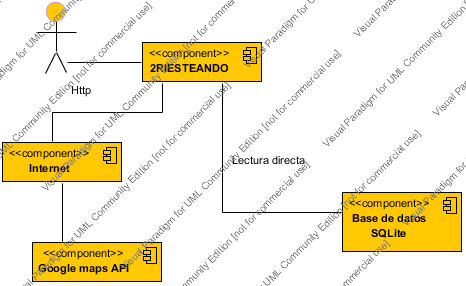
\includegraphics[width=14cm,height=6cm]{Imagenes/Despliegue/Arquitectonico.png}
  \caption{Diagrama de despliegue exterior}  
  \label{fig:arqui}
\end{figure}

El sistema interactuar\'a con una base de datos creada en SQLite 3, escribiendo directamente en ella, por otra parte realizar\'a una conex\'on
a internet a trav\'es del protocolo Http para obtener informaci\'on de la API de Google Maps versi\'on 2. Como
se muestra en la figura ~\ref{fig:arqui}.


\begin{figure}[h]

  \centering
  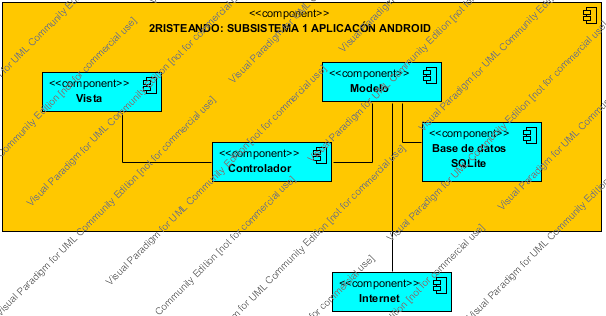
\includegraphics[width=18cm,height=6cm]{Imagenes/Despliegue/Subsistemas.png}
  \caption{Diagrama de despliegue interior}  
  \label{fig:subsistemas}
\end{figure}

El modelo de subsistemas est\'a representado en la figura ~\ref{fig:subsistemas}, el cual muestra el patr\'on de dise\~no
Modelo Vista Controlador. Donde la Vista ser\'a todo el conjunto de Activities que tendr\'a el sistema, el Controlador son
los eventos que controlar\'an la interacci\'on entre el Modelo y la Vista, finalmente, el Modelo tendra todo el funcionamiento
principal del sistema, como es calcular la ruta dependiendo el itinerario elegido o calcular un presupuesto seg\'un el n\'umero de personas
que asistan a dicha visita, interactuando con la base de datos que contiene el conjunto de informaci\'on de los lugares tur\'isticos
y la informaci\'on de los medios de transporte que pueden ser utilizados, as\'i como la interacc\'on con la API de Google Maps
para desplegar el mapa de la ciudad con los lugares seleccionados en el itinarario. 
	\newpage
			\section{Modelo del comportamiento}
  El sistema se encuentra organizado en un m\'odulo en el cual se destacan 3 acciones principales como se muestra en la figura 3:
  \begin{enumerate}
   \item Calcular ruta.
   \item Administrar Itinerario.
   \item Cambiar el idioma
  \end{enumerate}
  \begin{figure}[h]
      \centering
      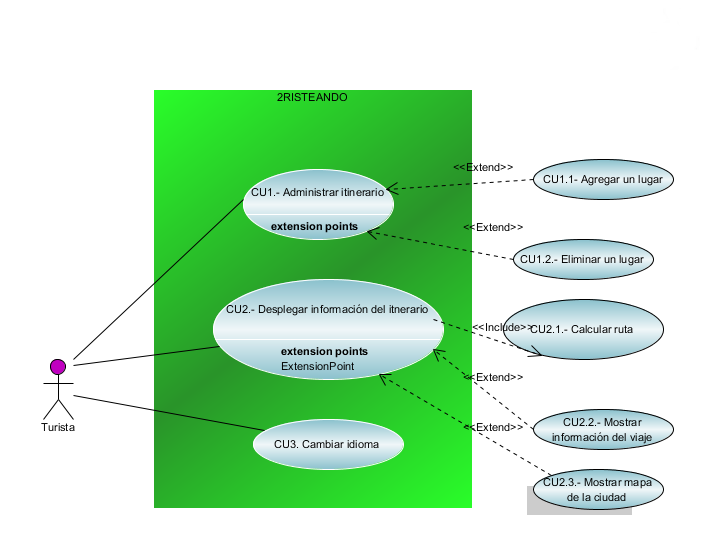
\includegraphics[width=12cm,height=10cm]{Imagenes/CasosUso/CU.png}
      \caption{Diagrama de casos de uso} 
      \label{fig:CU}
  \end{figure}
  
   \subsection{Actores del sistema}
    \subsubsection{Modelado de Actores}
    En esta secci\'on se describen las actividades que el Usuario podr\'a realizar.
    La figura siguiente muestra el perfil del Usuario que tendr\'a el sistema.
    
      \begin{figure}[h]
	\centering
	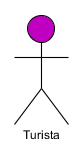
\includegraphics[width=2cm,height=3cm]{Imagenes/CasosUso/ActorTurista.PNG}
	\caption{Diagrama de actores del sistema}
	\label{fig:actores}
      \end{figure}
      
      
    \textbf{Nombre:} Turista
    \\
    \\
    \textbf{Descripci\'on:} El turista es la persona ingresar\'a al sistema para buscar un lugar de su interes en la zona centro del D.F. 
    Pede elegir entre 3 diferentes idiomas ingl\'es, frances y espa\~nol. Elegir\'a entre el itinerario generado por el sistema
    o personalizar\'a el suyo. Finalmente podr\'a evaluar el calculo del presupuesto ofrecido por el sistema.
    \\
    \\
    \textbf{Cantidad:} Uno por dispositivo m\'ovil.
    
 \subsection{Casos de Uso}
  En esta secci\'on se describen los casos de uso de la figura ~\ref{fig:CU}. De cada uno se detallar\'an los siguientes elementos:
  \begin{itemize}
   \item \textbf{Resumen:} Decripci\'on textual del caso de uso.
   \item \textbf{Actores:} Lista de actores que intervienen en el caso de uso.
   \item \textbf{Porp\'osito:} Una breve descripci\'on del objetivo que busca el actor al ejecutar el caso de uso.
   \item \textbf{Entradas:} Lista de datos de entrada requeridos durante la ejecuci\'on del caso de uso.
   \item \textbf{Salidas:} Lista de los datos de salida que otorga el sistema durante la ejecuci\'on del caso de uso.
   \item \textbf{Precondiciones:} Descripci\'on de las operaciones o condiciones que se deben cumplir para
   que el caso de uso pueda ejecutarse correctamente.
   \item \textbf{Postcondiciones:} Lista de los cambios que ocurrir\'an en el sistema despu\'es de la ejecuci\'on
   del caso de uso.
   \item \textbf{Errores:} Lista de los posibles errores que pueden surgir durante la ejecuci\'on del caso de uso.
   \item \textbf{Trayectorias:} Secuencia de pasos que ejecutar\'a el caso de uso.
  \end{itemize}



 
	\newpage
			\subsection{Trayectorias}
  \subsubsection{CU1 Desplegar informaci\'on}
  \textbf{Resumen}
  \\
  \\
    El actor podr\'a visualizar la informaci\'on del itinerario elegido, esto es el mapa del transporte elegido, la descripci\'on de manera escrita
    de la ruta a seguir en el medio de transporte, el c\'alculo del presupuesto si as� lo requiere y un mapa de la ciudad con los lugares marcados
    de su itinerario para poder guiarse y llegar a pie.
  \\
  \\
  
  \textbf{Descripci\'on}
  \\
  \\
  \begin{tabular}{|p{3.5cm}|p{12cm}|l|}
     \hline
     \textbf{Caso de Uso:} & CU1 Desplegar informaci\'on \\ \hline
     \textbf{Actor:} & Turista\\ \hline
     \textbf{Prop\'osito:} & Visualizar la informaci�n del itinerario elegido\\ \hline
     \textbf{Entradas:} & -\\ \hline
     \textbf{Salidas: } & Por default muestra el mapa de la ruta del transporte.\\ \hline
     \textbf{Precondiciones: } & Un itinerario establecido.\\ \hline
     \textbf{Postcondiciones: } & - \\ \hline
     \textbf{Errores: } & -\\ \hline
     \textbf{Tipo:} & Prinario.\\ \hline
   \end{tabular}
   
   \subsubsection{Trayectoria Principal}
      \begin{enumerate}
	\item El \textbf{Actor} ingresa en la pantalla [VCU1.1].
	\item El \textbf{Sistema} carga la primer pesta�a de mostrar el mapa
	\item El \textbf{Sistema} muestra la pantalla de despliegue de informaci\'on con las siguientes opciones:
	\begin{itemize}
	 \item Calcular ruta.[PE CU1.1]
	 \item Mostrar informaci\'on del viaje. [PE CU1.2]
	 \item Mostrar mapa de la ciudad. [PE CU1.3]
	\end{itemize}
      \end{enumerate}	   
      --Fin del caso de uso.
      
\newpage
  \subsubsection{CU1.1 Calcular ruta}
  \textbf{Resumen}
  \\
  \\
    El sistema toma las coordenadas del turista y del destino base, por medio del GPS para calcular la ruta que llevar\'a al(los) turista(s)
    a la estaci\'on m\'as cercana del primer lugar de su itinerario, utilizando ya sea el metro o metrobus, dependindo de la elecci\'on del turista.
  \\
  \\
  
  \textbf{Descripci\'on}
  \\
  \\
  \begin{tabular}{|p{3.5cm}|p{12cm}|l|}
     \hline
     \textbf{Caso de Uso:} & CU1.1 Calcular ruta \\ \hline
     \textbf{Actor:} & Turista\\ \hline
     \textbf{Prop\'osito:} & Calcular la ruta para llegar al destino base.\\ \hline
     \textbf{Entradas:} & Las coordenadas del destino base, ubicaci\'on del turista, mediante el GPS
     y el medio de transporte a utilizar, seleccion\'andolo en un combobox\\ \hline
     \textbf{Salidas: } & El mapa del transporte seleccionado, con la ruta dibujada, que seguir\'a el
     usuario para llegar al destino base.\\ \hline
     \textbf{Precondiciones: } & El GPS del celular est\'a activado; La conexi\'on internet est\'a funcionando. Debe existir al menos un lugar destino y un
     cat\'alogo de transportes a utilizar.\\ \hline
     \textbf{Postcondiciones: } & - \\ \hline
     \textbf{Errores: } & [MSG4] Fallo en la conexi\'on de la Base de Datos. [MSG1] Informaci\'on incompleta.\\ \hline
     \textbf{Tipo:} & Secundario.\\ \hline
   \end{tabular}
   
   \subsubsection{Trayectoria Principal}
      \begin{enumerate}
	\item El \textbf{Actor} ingresa en la pantalla [VCU2].
	\item El \textbf{Actor} selecciona al menos un lugar a visitar.
	\item El \textbf{Actor} selecciona del combobox el medio de transporte que utilizar\'a.
	\item El \textbf{Actor} pulsa el bot\'on \textbf{Siguiente}.
	\item El \textbf{Sistema} valida que exista por lo menos un lugar a visitar.[Trayectoria Alternativa A]
	\item El \textbf{Sistema} calcula la ruta seg\'un el transporte seleccionado y el detino base. [Trayectoria Alternativa B]
	\item El \textbf{Sistema} muestra el mapa del transporte elegido, con la ruta a seguir para llegar
	a la estaci\'on m\'as cercana del destino base de la vista [VCU1.1].
      \end{enumerate}	   
      --Fin del caso de uso.
    
    \subsubsection{Trayectoria Alternativa A}
	\textbf{Condici\'on: } El turista no seleccion\'o por lo menos un lugar a visitar.
	 \begin{enumerate}
	      \item El \textbf{Actor} pulsa en el bot\'on \textbf{Siguiente}.
	      \item El \textbf{Sistema} valida que exista por lo menos un lugar a visitar.
	      \item El \textbf{Sistema} muestra el mensaje de error [MSG1] Informaci\'on incompleta,
	      mostrando el texto ``Falta llenar el campo Itinerario. Es obligatorio.''.
	      \item El \textbf{Actor} pulsa el bot\'on \textbf{Aceptar} del mensaje.
	      \item El \textbf{Sistema} regresa al paso 2 de la trayectoria principal.
	  \end{enumerate}
    --Fin de la trayectoria.
    
    \subsubsection{Trayectoria Alternativa B}
	\textbf{Condici\'on: } El sistema tuvo alg\'un problema con la conexi\'on de la base de datos.
	 \begin{enumerate}
	      \item El \textbf{Actor} hace clic en el bot\'on \textbf{Siguiente}.
	      \item El \textbf{Sistema} detecta un error en la conexi\'on de la base de datos.
	      \item El \textbf{Sistema} muestra el mensaje de error [MSG4] ``Error en la conexi\'on de la base de datos.''.
	      \item El \textbf{Actor} pulsa el bot\'on \textbf{Aceptar} del mensaje.
	      \item El \textbf{Sistema} regresa al paso 1 de la trayectoria principal.
	  \end{enumerate}
    --Fin de la trayectoria.
  
\newpage
    \subsubsection{CU1.2 Mostrar informaci\'on del viaje}
  \textbf{Resumen}
  \\
  \\
      El sistema calcular\'a el monto aproximado que se requiere para transportarse y visitar cada uno de los lugares en el itinerario
      selecionado, as\'i como mostrar de forma escrita la ruta que seguir\'a el turista en un medio de transporte seleccionado.
  \\
  \\
  
  \textbf{Descripci\'on}
  \\ 
  \\
  \begin{tabular}{|p{3.5cm}|p{12cm}|l|}
     \hline
     \textbf{Caso de Uso:} & CU1.2 Mostrar informaci\'on del viaje \\ \hline
     \textbf{Actor:} & Turista\\ \hline
     \textbf{Prop\'osito:} & Calcular el presupuesto del itinerario y mostrar la ruta de forma escrita.\\ \hline
     \textbf{Entradas:} & El n\'umero de personas ingresado en un campo de texto.\\ \hline
     \textbf{Salidas: } & El presupuesto total aproximado y la ruta de manera escrita.\\ \hline
     \textbf{Precondiciones: } & Un itinerario con los lugares a visitar (museos o restaurantes), la lista de precios de los lugares, as�
     como del transporte a utilizar. \\ \hline
     \textbf{Postcondiciones: } & - \\ \hline
     \textbf{Errores: } & [MSG4] Fallo en la conexi\'on de la Base de Datos. [MSG1] Informaci\'on incompleta.\\ \hline
     \textbf{Tipo:} & Secundario.\\ \hline
   \end{tabular}
   
   \subsubsection{Trayectoria Principal}
      \begin{enumerate}
	\item El \textbf{Actor} ingresa en la pantalla [VCU1.2].
	\item El \textbf{Sistema} despliega la ruta a seguir de forma escrita.
	\item El \textbf{Actor} ingresa el n\'umero de personas para realizar el c\'alculo
	del presupuesto del itinerario elegido.
	\item El \textbf{Actor} pulsa el bot\'on \textbf{Calcular presupuesto}.[Trayectoria Alternativa A]
	\item El \textbf{Sistema} realiza el calculo del presupuesto para el n\'umero de personas
	ingresado.[Trayectoria Alternativa B]
	\item El \textbf{Sistema} muestra el presupuesto total y por persona junto a la descripci\'on
	de la ruta del itinerario.

      \end{enumerate}	   
      --Fin del caso de uso.
    
    \subsubsection{Trayectoria Alternativa A}
	\textbf{Condici\'on: } El turista no ingres\'o el n\'umero de personas en el campo de texto
	para calcular el presupuesto.
	 \begin{enumerate}
	      \item El \textbf{Actor} pulsa en el bot\'on \textbf{Calcular presupuesto}.
	      \item El \textbf{Sistema} valida que se haya ingresado el n\'umero de personas para el presupuesto.
	      \item El \textbf{Sistema} muestra el mensaje de error [MSG1] Informaci\'on incompleta,
	      mostrando el texto ``Falta llenar el campo N\'umero de personas. Es obligatorio.''.
	      \item El \textbf{Actor} pulsa el bot\'on \textbf{Aceptar} del mensaje.
	      \item El \textbf{Sistema} regresa al paso 2 de la trayectoria principal.
	  \end{enumerate}
    --Fin de la trayectoria.
    
    \subsubsection{Trayectoria Alternativa B}
	\textbf{Condici\'on: } El sistema tuvo alg\'un problema con la conexi\'on de la base de datos.
	 \begin{enumerate}
	      \item El \textbf{Actor} hace clic en el bot\'on \textbf{Calcular presupuesto}.
	      \item El \textbf{Sistema} detecta un error en la conexi\'on de la base de datos.
	      \item El \textbf{Sistema} muestra el mensaje de error [MSG4] ``Error en la conexi\'on de la base de datos.''.
	      \item El \textbf{Actor} pulsa el bot\'on \textbf{Aceptar} del mensaje.
	      \item El \textbf{Sistema} regresa al paso 1 de la trayectoria principal.
	  \end{enumerate}
    --Fin de la trayectoria.
  
 \newpage
    \subsubsection{CU1.3 Mostrar mapa de la ciudad}
  \textbf{Resumen}
  \\
  \\
      El turista podr\'a visualizar el mapa de la ciudad, con los lugares de su itinerario marcados para poder tener una mejor
      referncia de como llegar y que calles se encuentran a su alrededor.
  \\
  \\
  
  \textbf{Descripci\'on}
  \\ 
  \\
  \begin{tabular}{|p{3.5cm}|p{12cm}|l|}
     \hline
     \textbf{Caso de Uso:} & CU1.3 Mostrar mapa de la ciudad \\ \hline
     \textbf{Actor:} & Turista\\ \hline
     \textbf{Prop\'osito:} & Visualizar el mapa de la ciudad con los lugares del itinerario.\\ \hline
     \textbf{Entradas:} & -\\ \hline
     \textbf{Salidas: } & El mapa con los lugares marcados\\ \hline
     \textbf{Precondiciones: } & Un itinerario previamente hecho. \\ \hline
     \textbf{Postcondiciones: } & - \\ \hline
     \textbf{Errores: } & [MSG8] Fallo en la conex\'on con google\\ \hline
     \textbf{Tipo:} & Secundario.\\ \hline
   \end{tabular}
   
    \subsubsection{Trayectoria Principal}
      \begin{enumerate}
	\item El \textbf{Actor} ingresa en la pantalla [VCU1.3] para visualizar el mapa de google.
	\item El \textbf{Sistema} se conecta con la API de google para mostrar el mapa.[Trayectoria Aleternativa A]
	\item El \textbf{Sistema} manda las coordenadas de los lugares para ubicarlas en el mapa.
	\item El \textbf{Sistema} despliega el mapa de la ciudad con los lugares ubicados.
      \end{enumerate}	   
      --Fin del caso de uso.
      \subsubsection{Trayectoria Alternativa A}
	\textbf{Condici\'on: } El sistema tuvo alg\'un problema con la conexi\'on de google.
	 \begin{enumerate}
	      \item El \textbf{Actor} hace clic en el bot\'on \textbf{Siguiente}.
	      \item El \textbf{Sistema} detecta un error en la conexi\'on de la base de datos.
	      \item El \textbf{Sistema} muestra el mensaje de error [MSG8] ``No se ha podido establecer conexi\'on.''.
	      \item El \textbf{Actor} pulsa el bot\'on \textbf{Aceptar} del mensaje.
	      \item El \textbf{Sistema} regresa al paso 1 de la trayectoria principal.
	  \end{enumerate}
    --Fin de la trayectoria.
    
    
  \newpage
  \subsubsection{CU2 Administrar itinerario}
  \textbf{Resumen}
  \\
  \\
  Le permitir\'a al usuario establecer el destino base y un radio m\'aximo de b\'usqueda de lugares cercanos
  para comenzar a crear su itinerario, a partir del destino base ingresado.
  \\
  \\
  
  \textbf{Descripci\'on}
  \\
  \\
  \begin{tabular}{|p{3.5cm}|p{12cm}|l|}
     \hline
     \textbf{Caso de Uso:} & CU2 Administrar itinerario \\ \hline
     \textbf{Actor:} & Turista\\ \hline
     \textbf{Prop\'osito:} & Establecer el destino base y el radio m\'aximo de b\'usqueda. \\ \hline
     \textbf{Entradas:} &  El turista ingresar\'a en un campo de texto el destino base, y en un numpicker
     el radio \'aximo para buscar los dem\'as lugares.\\ \hline
     \textbf{Salidas: } & Lista de los lugares posibles a visitar.\\ \hline
     \textbf{Precondiciones: } & Debe existir un cat\'alogo de lugares en la base de datos.\\ \hline
     \textbf{Postcondiciones: } & - \\ \hline
     \textbf{Errores: } & [MSG4] Fallo en la conexi\'on de la Base de Datos. [MSG1] Informaci\'on incompleta. [MSG7] Idioma no disponible.\\ \hline
     \textbf{Tipo:} & Primario.\\ \hline
   \end{tabular}
   
   \subsubsection{Trayectoria Principal}
      \begin{enumerate}
	\item El \textbf{Actor} ingresa en la pantalla [Vista Principal] para acceder al sistema.
	\item El \textbf{Sistema} valida el idioma del dispositivo m\'ovil respecto a la regla de negocio.
	[RN7].[Trayectoria Alternativa A]
	\item El \textbf{Actor} escribe en el campo de texto el destino base.
	\item El \textbf{Actor} establece un radio m\'aximo de b\'usqueda de lugares al rededor del destino base.
	\item El \textbf{Actor} pulsa el bot\'on de \textbf{Siguiente}.
	\item El \textbf{Sistema} valida la informaci\'on ingresada al sistema[Trayectoria alternativa B]
	\item El \textbf{Sistema} busca los lugares m\'as cercanos dependiendo del radio establecido. [Trayectoria Alternativa C]
      \end{enumerate}	   
      --Fin del caso de uso.
    
     \subsubsection{Trayectoria Alternativa A}
	\textbf{Condici\'on: } El sistema no encuentra el idioma del dispositivo m\'ovil en los disponibles para el sistema.
	 \begin{enumerate}
	      \item El \textbf{Actor} ingrsa a la pantalla [Vista Principal].
	      \item El \textbf{Sistema} valida el idioma del dispositivo m\'ovil.
	      \item El \textbf{Sistema} muestra el mensaje de error [MSG7] Idioma disponible.
	      \item El \textbf{Actor} pulsa el bot\'on \textbf{Aceptar} del mensaje.
	      \item El \textbf{Sistema} establece el idioma ingl\'es por default.
	      \item El \textbf{Sistema} regresa al paso 1 de la trayectoria principal.
	  \end{enumerate}
    --Fin de la trayectoria.
    
    \subsubsection{Trayectoria Alternativa B}
	\textbf{Condici\'on: } El turista no escribi\'o el destino base para realizar la b\'usqueda de los dem\'as lugares.
	 \begin{enumerate}
	      \item El \textbf{Actor} pulsa en el bot\'on \textbf{Siguiente}.
	      \item El \textbf{Sistema} valida que est\'e escrito el lugar destino en el campo de texto.
	      \item El \textbf{Sistema} muestra el mensaje de error [MSG1] Informaci\'on incompleta,
	      mostrando el texto ``Falta llenar el campo N\'umero de personas. Es obligatorio.''.
	      \item El \textbf{Actor} pulsa el bot\'on \textbf{Aceptar} del mensaje.
	      \item El \textbf{Sistema} regresa al paso 2 de la trayectoria principal.
	  \end{enumerate}
    --Fin de la trayectoria.
    
    \subsubsection{Trayectoria Alternativa C}
	\textbf{Condici\'on: } El sistema tuvo alg\'un problema con la conexi\'on de la base de datos.
	 \begin{enumerate}
	      \item El \textbf{Actor} hace clic en el bot\'on \textbf{Siguiente}.
	      \item El \textbf{Sistema} detecta un error en la conexi\'on de la base de datos.
	      \item El \textbf{Sistema} muestra el mensaje de error [MSG4] ``Error en la conexi\'on de la base de datos.''.
	      \item El \textbf{Actor} pulsa el bot\'on \textbf{Aceptar} del mensaje.
	      \item El \textbf{Sistema} regresa al paso 1 de la trayectoria principal.
	  \end{enumerate}
    --Fin de la trayectoria.
  
  \newpage
  \subsubsection{CU2.1 Agregar un lugar}
  \textbf{Resumen}
  \\
  \\
  Le permitir\'a al turista agregar a su itinerario un lugar tur\'istico o restaurante. El cual puedr\'a ser el punto
  de inicio para calcular la ruta de llegada.
  \\
  \\
  
  \textbf{Descripci\'on}
  \\
  \\
  \begin{tabular}{|p{3.5cm}|p{12cm}|l|}
     \hline
     \textbf{Caso de Uso:} & CU2.1 Agregar un lugar \\ \hline
     \textbf{Actor:} & Turista\\ \hline
     \textbf{Prop\'osito:} & Seleccionar lugares tur\'isticos o restaurante a un itinerario. \\ \hline
     \textbf{Entradas:} & Mediante un \textbf{checkbox} se crear\'a la lista de los lugares tur\'isticos
     y/o restaurantes a visitar por el turista.\\ \hline
     \textbf{Salidas: } & Listado de los lugares seleccionados. \\ \hline
     \textbf{Precondiciones: } & Debe existir el cat\'alogo de lugares tur\'isticos y restaurantes.\\ \hline
     \textbf{Postcondiciones: } & - \\ \hline
     \textbf{Errores: } & [MSG4] Fallo en la conexi\'on de la Base de Datos.,  [MSG5] Limite de lugares permitido. y [MSG6] M\'inimo de lugares seleccionado \\ \hline
     \textbf{Tipo:} & Segundario.\\ \hline
   \end{tabular}
   
   \subsubsection{Trayectoria Principal}
      \begin{enumerate}
	\item El \textbf{Actor} ingresa en la pantalla [VCU2.1].[Trayectoria Alternativa A]
	\item El \textbf{Sistema} se conecta a la base de datos. [Trayectoria Alternativa B]
	\item El \textbf{Sistema} muestra una lista de los lugares posibles a seleccionar.
	\item El \textbf{Actor} selecciona 5 lugares que desee visitar. [PE CU2.2] [Trayectoria Alternativa C]
	\item El \textbf{Actor} pulsa el bot\'on \textbf{Siguiente}.
	\item El \textbf{Sistema} muestra el mensaje [MSG3] Confirmaci\'on ``?`Seguro que desea calcular la ruta?''.[Trayectoria Alternativa D]
	\item El \textbf{Actor} pulsa el bot\'on \textbf{Aceptar} para confirmar su decisi\'on.
	\item El \textbf{Sistema} muestra la pantalla [VCU1].
      \end{enumerate}	   
      --Fin del caso de uso.
      
    \subsubsection{Trayectoria Alternativa A}
	\textbf{Condici\'on: } El turista decidi\'o cambiar de lugar tur\'istico base.
	 \begin{enumerate}
	      \item El \textbf{Actor} hace clic en el bot\'on \textbf{Atr\'as}.
	      \item El \textbf{Sistema} regresa a va pantalla [Vista principal del sistema].
	  \end{enumerate}
    --Fin del caso de uso. 
    
    \subsubsection{Trayectoria Alternativa B}
	\textbf{Condici\'on: } El sistema tuvo alg\'un problema con la conexi\'on de la base de datos.
	 \begin{enumerate}
	      \item El \textbf{Actor} hace clic en el bot\'on \textbf{Siguiente}.
	      \item El \textbf{Sistema} detecta un error en la conexi\'on de la base de datos.
	      \item El \textbf{Sistema} muestra el mensaje de error [MSG4] ``Error en la conexi\'on de la base de datos.''.
	      \item El \textbf{Actor} pulsa el bot\'on \textbf{Aceptar} del mensaje.
	      \item El \textbf{Sistema} regresa al paso 1 de la trayectoria principal.
	  \end{enumerate}
    --Fin de la trayectoria.
    
    \subsubsection{Trayectoria Alternativa C}
	\textbf{Condici\'on: } El actor no seleccion\'o alg\'un lugar para visitar.
	 \begin{enumerate}
	      \item El \textbf{Actor} pulsa el bot\'on \textbf{Siguiente}.
	      \item El \textbf{Sistema} muestra el mensaje de error [MSG6] ``Error, debes seleccionar al menos 1 lugar.''.
	      \item El \textbf{Actor} pulsa el bot\'on \textbf{Aceptar}.
	      \item El \textbf{Sistema} regresa al paso 4 de la trayectoria principal.
	  \end{enumerate}
    --Fin de la trayectoria.
    
        \subsubsection{Trayectoria Alternativa D}
	\textbf{Condici\'on: } El actor decidi\'o cambiar su itinerario.
	 \begin{enumerate}
	      \item El \textbf{Actor} hace clic en el bot\'on \textbf{Cancelar}.
	      \item El \textbf{Sistema} regresa al paso n\'umero 4 de la trayectoria principal.
	  \end{enumerate}
    --Fin de la trayectoria.
  
 \newpage
 \subsubsection{CU2.2 Eliminar un lugar}
  \textbf{Resumen}
  \\
  \\
  El turista podr\'a decidir quitar un lugar del itinerario que ha creado.
  \\
  \\
  
  \textbf{Descripci\'on}
  \\
  \\
  \begin{tabular}{|p{3.5cm}|p{12cm}|l|}
     \hline
     \textbf{Caso de Uso:} & CU2.2 Eliminar un lugar \\ \hline
     \textbf{Actor:} & Turista\\ \hline
     \textbf{Prop\'osito:} & Quitar lugares tur\'isticos del itinerario. \\ \hline
     \textbf{Entradas:} & Un itinerario con por lo menos 1 lugar tur\'istico \\ \hline
     \textbf{Salidas: } & Una lista con menor n\'umero de lugares tur\'isticos en el itinerario. \\ \hline
     \textbf{Precondiciones: } & Debe haberse elegido por lo menos un lugar tur\'istico. \\ \hline
     \textbf{Postcondiciones: } & - \\ \hline
     \textbf{Errores: } & - \\ \hline
     \textbf{Tipo:} & Secundario.\\ \hline
   \end{tabular}
   
   \subsubsection{Trayectoria Principal}
      \begin{enumerate}
	\item El \textbf{Actor} ingresa en la pantalla [VCU2.2].[Trayectoria Alternativa A]
	\item El \textbf{Sistema} muestra la lista de los lugares seleccionados.
	\item El \textbf{Actor} pulsa el bot\'on con una \textbf{X} para quitar un lugar tur\'istico.
	\item El \textbf{Sistema} muestra un lugar tur\'istico menos en el itinerario.
      \end{enumerate}	   
      --Fin del caso de uso.
      
    \subsubsection{Trayectoria Alternativa A}
	\textbf{Condici\'on: } El turista decidi\'o cambiar de lugar tur\'istico base.
	 \begin{enumerate}
	      \item El \textbf{Actor} hace clic en el bot\'on \textbf{Atr\'as}.
	      \item El \textbf{Sistema} regresa a va pantalla [Vista Principal].
	  \end{enumerate}
    --Fin del caso de uso.

\newpage
  
  \subsubsection{CU3 Cambiar idioma}
  \textbf{Resumen}
  \\
  \\
	La informaci\'on contenida en la aplicaci\'on ser\'a mostrada al usuario en uno de los 3 idiomas disponibles:
	\begin{enumerate}
	  \item Espa\~nol
	  \item Ingles
	  \item Frances
	\end{enumerate}
  
  
  \textbf{Descripci\'on}
  \\
  \\
  \begin{tabular}{|p{3.5cm}|p{12cm}|l|}
     \hline
     \textbf{Caso de Uso:} & CU3 Cambiar idioma \\ \hline
     \textbf{Actor:} & -\\ \hline
     \textbf{Prop\'osito:} & Mostrar la informaci\'on de la aplicaci\'on como m\'as le agrade al usuario. \\ \hline
     \textbf{Entradas:} & El el idioma seleccionado por el usuario. \\ \hline
     \textbf{Salidas: } & El texto de informaci\'on de la aplicaci\'on se mostrar\'a en el idioma selccionado. \\ \hline
     \textbf{Precondiciones: } &  -\\ \hline
     \textbf{Postcondiciones: } & - \\ \hline
     \textbf{Errores: } & [MSG4] Fallo en la conexi\'on de la Base de Datos.\\ \hline
     \textbf{Tipo:} & Primario.\\ \hline
   \end{tabular}
   
   \subsubsection{Trayectoria Principal}
      \begin{enumerate}
	\item El \textbf{Actor} ingresa en la pantalla [VCU3].
	\item El \textbf{Actor} selecciona el idioma de su preferencia.
	\item El \textbf{Actor} pulsa el bot\'on \textbf{Cambiar idioma}{Trayectoria Aleternativa A}
	\item El \textbf{Sistema} configura el idioma seleccionado por el usuario.

      \end{enumerate}	   
      --Fin del caso de uso.
      
    \subsubsection{Trayectoria Alternativa A}
	\textbf{Condici\'on: } El sistema tuvo alg\'un problema con la conexi\'on de la base de datos.
	 \begin{enumerate}
	      \item El \textbf{Actor} hace clic en el bot\'on \textbf{Cambiar idioma}.
	      \item El \textbf{Sistema} detecta un error en la conexi\'on de la base de datos.
	      \item El \textbf{Sistema} muestra el mensaje de error [MSG4] ``Error en la conexi\'on de la base de datos.''.
	      \item El \textbf{Actor} pulsa el bot\'on \textbf{Aceptar} del mensaje.
	      \item El \textbf{Sistema} regresa al paso 1 de la trayectoria principal.
	  \end{enumerate}
    --Fin de la trayectoria.
  
	\newpage
			\section{Modelo del dominio del problema}
\begin{figure}[h]

	\subsection{Modelo est\'atico}
		\subsubsection{Diagrama de clases}
		  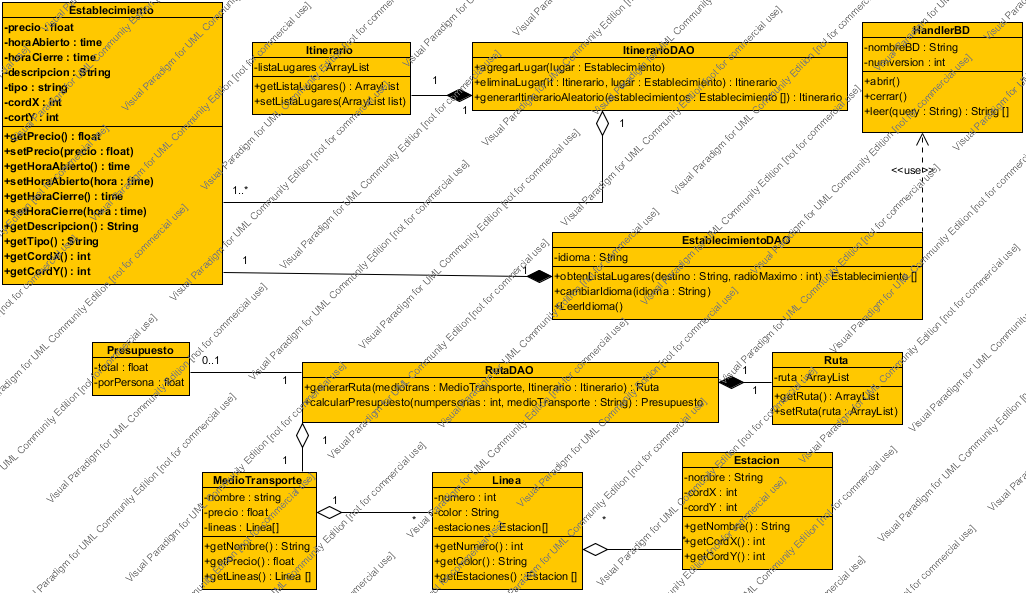
\includegraphics[width=18cm,height=8cm]{Imagenes/DiagramaClases/Estatico.png}
		\subsubsection{Diagramas entidad-relaci\'on}
		  %%\centering
			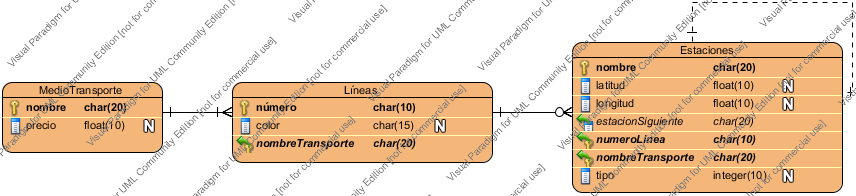
\includegraphics[width=18cm,height=6cm]{Imagenes/BasedeDatos/2RISTEANDODB.png}
		  %%\caption{Diagrama Entidad-Realci\'on}
	\subsection{Modelo din\'atico}
		\subsubsection{Diagrama de clases}
		\subsubsection{Diagramas de secuencias}
  

\end{figure}
  
 
	\newpage
			\section{Modelo de interfaces}
En esta secci\'on se describen las pantallas que componen el sistema,
mostrando los campos que componen los formularios, as\'i como los mensjaes
de ayuda o error que puedan presentarse a lo largo de la ejecuci\'on.

\subsection{Ingreso al sistema}

\begin{figure}[h]
  \centering
    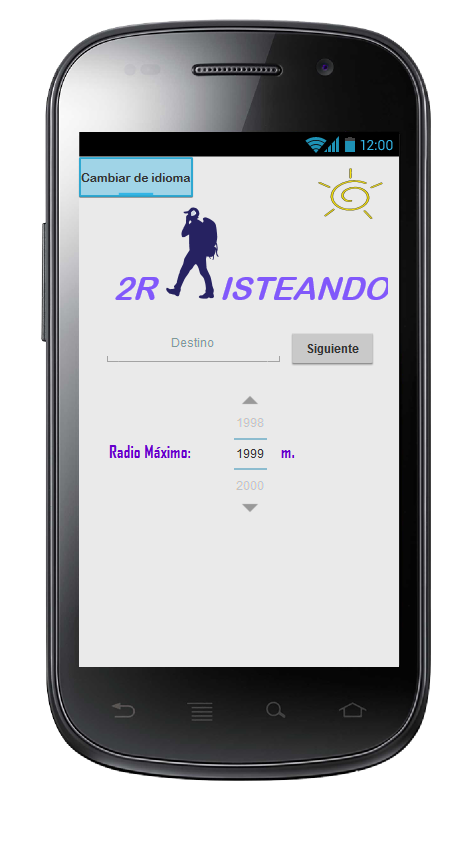
\includegraphics[width=5cm,height=8cm]{Imagenes/VistasSistema/VistaPrincipal.png}
  \caption{Vista principal del sistema.}  
\end{figure}

\newpage
\subsection{Despliegue de informaci\'on}
\begin{figure}[h]
  \centering
    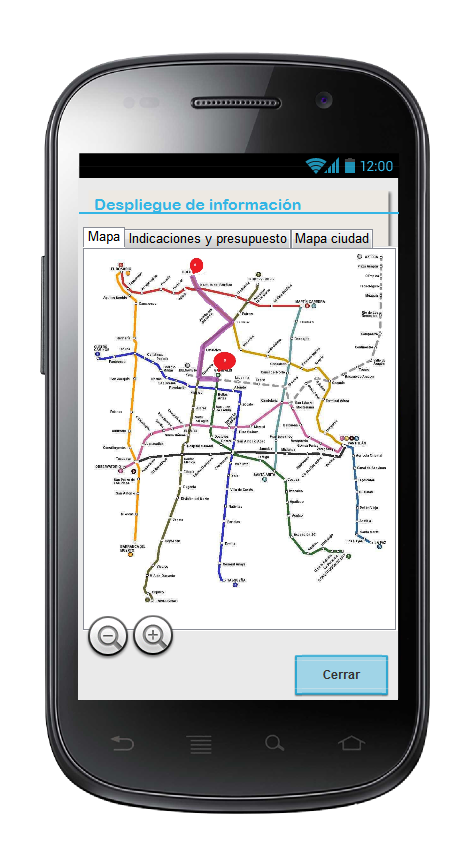
\includegraphics[width=5cm,height=8cm]{Imagenes/VistasSistema/CU1_1.png}
  \caption{VCU1.1 Vista para ver la ruta en el medio de transporte.}  
\end{figure}

\begin{figure}[h]
  \centering
    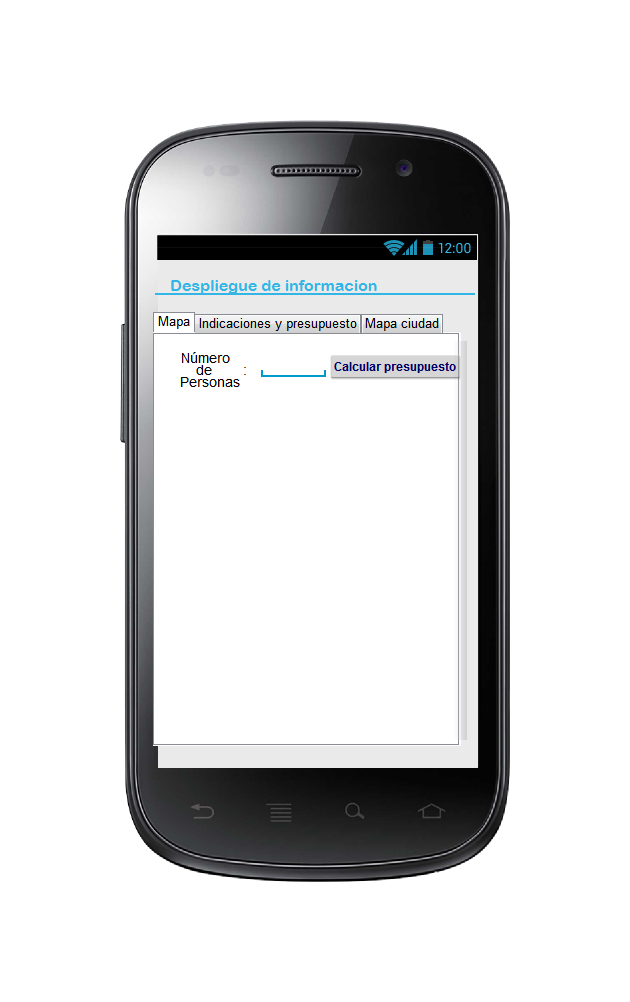
\includegraphics[width=5cm,height=8cm]{Imagenes/VistasSistema/CU1_2.png}
  \caption{VCU1.2 Vista para ver informaci\'on del viaje}  
\end{figure}

\begin{figure}[h]
  \centering
    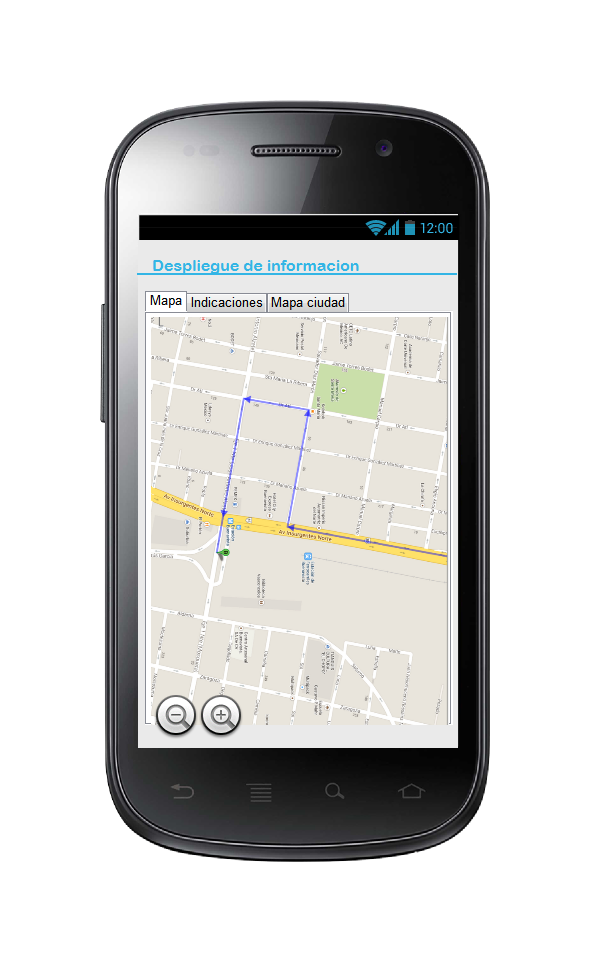
\includegraphics[width=5cm,height=8cm]{Imagenes/VistasSistema/CU1_3.png}
  \caption{VCU1.3 Vista para ver el mapa de la ciudad}  
\end{figure}

\newpage
\subsection{Administrar el itinerario}

\begin{figure}[h]
  \centering
    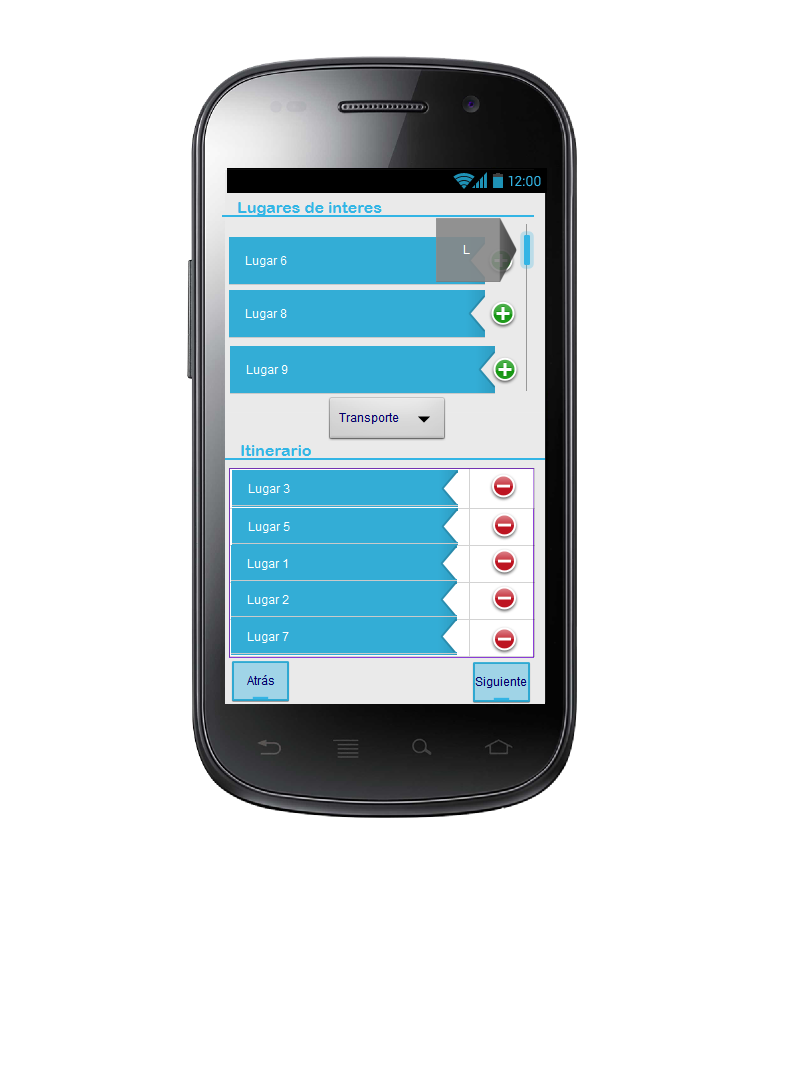
\includegraphics[width=5cm,height=8cm]{Imagenes/VistasSistema/CU2.png}
  \caption{VCU2 Vista para administrar el itinerario.}  
\end{figure}

\newpage
\subsection{Agregar un lugar}

\begin{figure}[h]
  \centering
    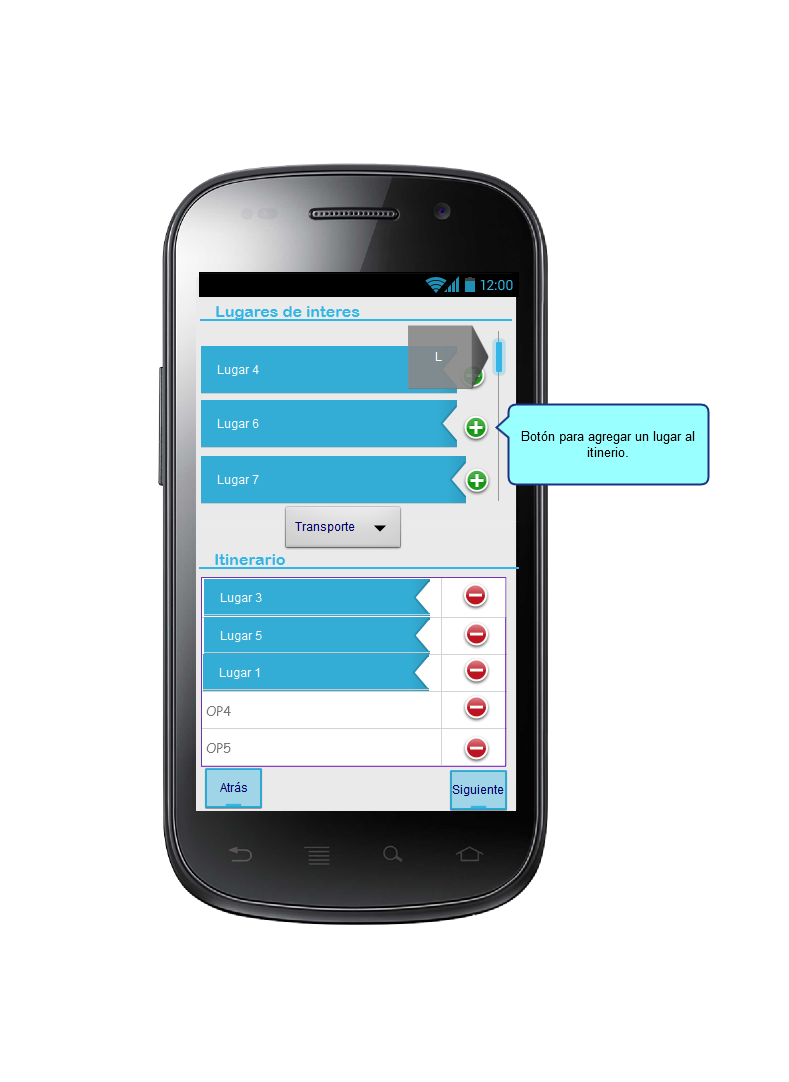
\includegraphics[width=5cm,height=8cm]{Imagenes/VistasSistema/CU2_1.png}
  \caption{VCU2.1 Vista para agregar un lugar al itinerario.}  
\end{figure}

\newpage
\subsection{Eliminar un lugar}

\begin{figure}[h]
  \centering
    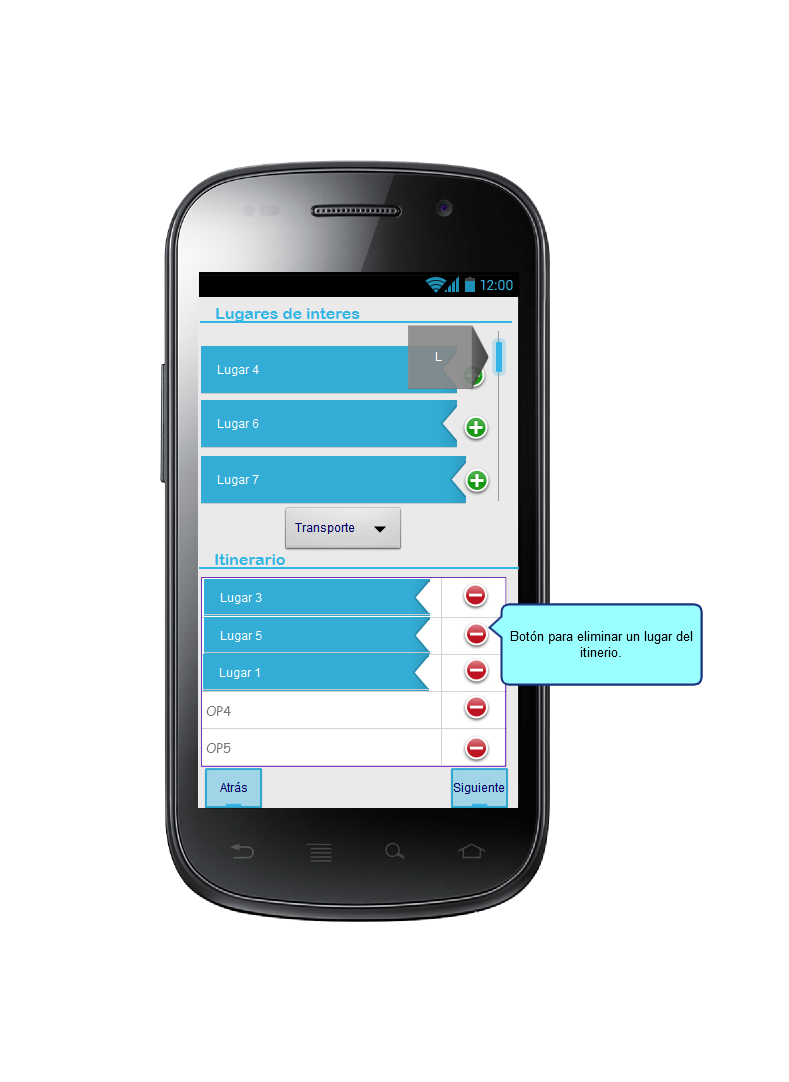
\includegraphics[width=5cm,height=8cm]{Imagenes/VistasSistema/CU2_2.png}
  \caption{VCU2.1 Vista para eliminar un lugar al itinerario.}  
\end{figure}

\newpage
\subsection{Cambiar idioma}

\begin{figure}[h]
  \centering
    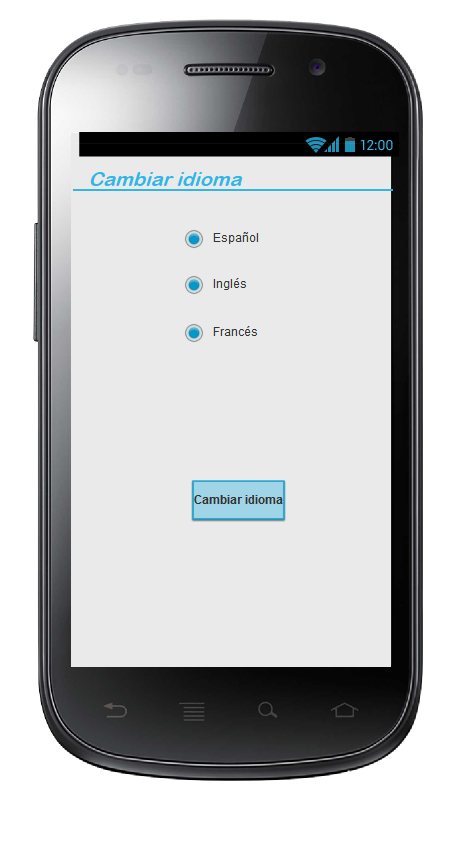
\includegraphics[width=5cm,height=8cm]{Imagenes/VistasSistema/CU3.png}
  \caption{VCU3 Vista para cambiar el idioma del sistema.}  
\end{figure}

   	
	\newpage
			\section{Reglas de negocio}

 \begin{table}[h]
    \begin{tabular}{|p{3.5cm}|p{10cm}|l|}
     \hline
     \textbf{Regla: } & RN1 N\'umero de lugares tur\'isticos en el itinerario\\ \hline
     \textbf{Tipo: } & Restricci\'on \\ \hline
     \textbf{Nivel:} & Alto \\ \hline
     \textbf{Versi\'on: } & 1.0 \\ \hline
     \textbf{Estado: } & En revisi\'on \\ \hline
     \textbf{Descripci\'on: } & Solo se podr\'an asignar m\'inimo 1 y m\'aximo 5 lugares tur\'isticos en el itinerario \\ \hline
     \textbf{Referenciada por: } & - \\
     \hline
   \end{tabular}
\end{table}

 \begin{table}[h]
    \begin{tabular}{|p{3.5cm}|p{10cm}|l|}
     \hline
     \textbf{Regla: } & RN2 Lugares tur\'isticos\\ \hline
     \textbf{Tipo: } & Restricci\'on \\ \hline
     \textbf{Nivel:} & Alto \\ \hline
     \textbf{Versi\'on: } & 1.0 \\ \hline
     \textbf{Estado: } & En revisi\'on \\ \hline
     \textbf{Descripci\'on: } & El cat\'alogo de museos solo ser\'a de 30 museos. \\ \hline
     \textbf{Referenciada por: } & - \\
     \hline
   \end{tabular}
\end{table}

 \begin{table}[h]
    \begin{tabular}{|p{3.5cm}|p{10cm}|l|}
     \hline
     \textbf{Regla: } & RN3 Restaurantes\\ \hline
     \textbf{Tipo: } & Restricci\'on \\ \hline
     \textbf{Nivel:} & Alto \\ \hline
     \textbf{Versi\'on: } & 1.0 \\ \hline
     \textbf{Estado: } & En revisi\'on \\ \hline
     \textbf{Descripci\'on: } & Solo se mostrar\'an lugares de comida Vips y MCdonald's. \\ \hline
     \textbf{Referenciada por: } & - \\
     \hline
   \end{tabular}
\end{table}

 \begin{table}[h]
    \begin{tabular}{|p{3.5cm}|p{10cm}|l|}
     \hline
     \textbf{Regla: } & RN4 Rutas de Transporte\\ \hline
     \textbf{Tipo: } & Restricci\'on \\ \hline
     \textbf{Nivel:} & Alto \\ \hline
     \textbf{Versi\'on: } & 1.0 \\ \hline
     \textbf{Estado: } & En revisi\'on \\ \hline
     \textbf{Descripci\'on: } & Solo se usar\'a el Metro y el Metrobus como medio de transporte para
     acercar al usuario a su destino base. \\ \hline
     \textbf{Referenciada por: } & - \\
     \hline
   \end{tabular}
  \end{table} 
\begin{table}[h]
    \begin{tabular}{|p{3.5cm}|p{10cm}|l|}
     \hline
     \textbf{Regla: } & RN5 Trazado de la ruta\\ \hline
     \textbf{Tipo: } &  Derivaci\'on\\ \hline
     \textbf{Nivel:} & Alto \\ \hline
     \textbf{Versi\'on: } & 1.0 \\ \hline
     \textbf{Estado: } & En revisi\'on \\ \hline
     \textbf{Descripci\'on: } & La ruta sera trazada por el sistema utilizando un 
     grafo recorriendo el menor n\'umero de estaciones en un solo sistema ya sea metro o 
     metrobus sin pasar por el mismo nodo m\'as de una vez. Como se muestra en la figura. 
     Se trazar\'a la ruta solamente desde el origen  hasta el destino base.\\ \hline 
     \textbf{Referenciada por: } & - \\
     \hline
   \end{tabular}
\end{table}

\begin{table}[h]
    \begin{tabular}{|p{3.5cm}|p{10cm}|l|}
     \hline
     \textbf{Regla: } & RN6 C\'alculo de presupuesto\\ \hline
     \textbf{Tipo: } &  Restricci\'on\\ \hline
     \textbf{Nivel:} & Alto \\ \hline
     \textbf{Versi\'on: } & 1.0 \\ \hline
     \textbf{Estado: } & En revisi\'on \\ \hline
     \textbf{Descripci\'on: } & El presupuesto para el itinerario a seguir se calcular\'a de la siguiente
     manera: se multiplicar\'a el n\'umero de personas por la suma del costo de cada establecimiento. Sin tomar
     en cuenta los descuentos que se puedan dar en el metro o museos. Finalmente se desplegara el presupuesto total
     y por persona.\\ \hline 
     \textbf{Referenciada por: } & - \\
     \hline
   \end{tabular}
\end{table}

\begin{table}[h]
    \begin{tabular}{|p{3.5cm}|p{10cm}|l|}
     \hline
     \textbf{Regla: } & RN7 Idiomas\\ \hline
     \textbf{Tipo: } &  Restricci\'on\\ \hline
     \textbf{Nivel:} & Alto \\ \hline
     \textbf{Versi\'on: } & 1.0 \\ \hline
     \textbf{Estado: } & En revisi\'on \\ \hline
     \textbf{Descripci\'on: } & Cuando el idioma del dispositivo m\'ovil no sea compatible con el sistema, el sitema elegir\'a por default
     el idioma ingl\'es para mostrar toda la informaci\'on.\\ \hline 
     \textbf{Referenciada por: } & - \\
     \hline
   \end{tabular}
\end{table}
	\newpage
			%*******************Errores*******************************
\section{Mensajes}

\begin{table}[ht]
   \begin{tabular}{|p{3cm}|p{12cm}|l|}
     \hline
     \textbf{MSG1 } &  Informaci\'on incompleta\\ \hline
     \textbf{Tipo } & Error \\ \hline
     \textbf{Estatus} & En revisi\'on \\ \hline
     \textbf{Objetivo } &  Mostrar al usuario que le falta un campo obligatorio por llenar\\ \hline
     \textbf{Redacci\'on } & Falta llenar el campo NOMBRE\_CAMPO. Es obligatorio\\ \hline
     \textbf{Par\'ametros } &  NOMBRE\_CAMPO: Nombre del campo que se encuentra vacio. \\ 
				 \hline
     \textbf{Ejemplo} & Falta llenar el campo Nombre. Es obligatorio.\\
     \hline
   \end{tabular}
\end{table}

\begin{table}[ht]
   \begin{tabular}{|p{3cm}|p{12cm}|l|}
     \hline
     \textbf{MSG2 } & Resultado vac\'io\\ \hline
     \textbf{Tipo } & Error \\ \hline
     \textbf{Estatus} & En revisi\'on \\ \hline
     \textbf{Objetivo } & Avisar al usuario cuando el resultado de una consulta fu\'e vac\'io\\ \hline
     \textbf{Redacci\'on } & No se encontraron resultados\\ \hline
     \textbf{Par\'ametros } & -\\ \hline
     \textbf{Ejemplo} & No se encontraron resultados.\\
     \hline
   \end{tabular}
\end{table}

%*******************Alertas*******************************
\begin{table}[ht]
   \begin{tabular}{|p{3cm}|p{12cm}|l|}
     \hline
     \textbf{MSG3 } & Confirmaci\'on\\ \hline
     \textbf{Tipo } & Alerta \\ \hline
     \textbf{Estatus} & En revisi\'on \\ \hline
     \textbf{Objetivo } & Indicar si se aprueba alg\'un suceso a ocurrir\\ \hline
     \textbf{Redacci\'on } & ?`Seguro que desea ACCI\'ON?\\ \hline
     \textbf{Par\'ametros } & ACCI\'ON: Breve explicaci\'on de la acci\'on que ocurrir\'a\\ \hline
     \textbf{Ejemplo} & ?`Seguro que desea calcular la ruta?\\
     \hline
   \end{tabular}
\end{table}

%*******************Mensajes*******************************
\begin{table}[ht]
   \begin{tabular}{|p{3cm}|p{12cm}|l|}
     \hline
     \textbf{MSG4 } & Fallo en la conexi\'on de la base de datos\\ \hline
     \textbf{Tipo } & Error \\ \hline
     \textbf{Estatus} & En revisi\'on \\ \hline
     \textbf{Objetivo } & Mostrar al usuario que hay un problema con la conex\'on en la base de datos\\ \hline
     \textbf{Redacci\'on } & Error en la conexi\'on de la base de datos \\ \hline
     \textbf{Par\'ametros } & -\\ \hline
     \textbf{Ejemplo} & Error en la conexi\'on de la base de datos.\\
     \hline
   \end{tabular}
\end{table}

\begin{table}[ht]
   \begin{tabular}{|p{3cm}|p{12cm}|l|}
     \hline
     \textbf{MSG5 } & Limite de lugares permitido\\ \hline
     \textbf{Tipo } & Error \\ \hline
     \textbf{Estatus} & En revisi\'on \\ \hline
     \textbf{Objetivo } & Mostrarle al usuario cuando alcanz\'o el l\'imite de lugares permitidos\\ \hline
     \textbf{Redacci\'on } & Error, solo puedes seleccionar m\'aximo 5 lugares. \\ \hline
     \textbf{Par\'ametros } & -\\ \hline
     \textbf{Ejemplo} & Error, solo puedes seleccionar m\'aximo 5 lugares.\\
     \hline
   \end{tabular}
\end{table}

\begin{table}[ht]
   \begin{tabular}{|p{3cm}|p{12cm}|l|}
     \hline
     \textbf{MSG6 } & M\'inimo de lugares seleccionado\\ \hline
     \textbf{Tipo } & Error \\ \hline
     \textbf{Estatus} & En revisi\'on \\ \hline
     \textbf{Objetivo } & Mostrarle al usuario que no ha seleccionado al menos 1 lugar para su itinerario.\\ \hline
     \textbf{Redacci\'on } & Error, debes seleccionar al menos 1 lugar. \\ \hline
     \textbf{Par\'ametros } & -\\ \hline
     \textbf{Ejemplo} & Error, debes seleccionar al menos 1 lugar.\\
     \hline
   \end{tabular}
\end{table}

\begin{table}[ht]
   \begin{tabular}{|p{3cm}|p{12cm}|l|}
     \hline
     \textbf{MSG7 } & Idioma no disponible\\ \hline
     \textbf{Tipo } & Aviso \\ \hline
     \textbf{Estatus} & En revisi\'on \\ \hline
     \textbf{Objetivo } & Informarle al usuario que el idioma por default de su celular no es compatible con el sistema.\\ \hline
     \textbf{Redacci\'on } & El idioma de tu equipo no es compatible, el idioma del sistema por default ser\'a ingl\'es. \\ \hline
     \textbf{Par\'ametros } & -\\ \hline
     \textbf{Ejemplo} &  El idioma de tu equipo no es compatible, el idioma del sistema por default ser\'a ingl\'es.\\
     \hline
   \end{tabular}
\end{table}

\begin{table}[ht]
   \begin{tabular}{|p{3cm}|p{12cm}|l|}
     \hline
     \textbf{MSG8 } & Fallo en la conex\'on con google\\ \hline
     \textbf{Tipo } & Aviso \\ \hline
     \textbf{Estatus} & En revisi\'on \\ \hline
     \textbf{Objetivo } & Informarle al usuario que hay un prolema con la conexi�n con google\\ \hline
     \textbf{Redacci\'on } & No se ha podido establecer conexi\'on. \\ \hline
     \textbf{Par\'ametros } & -\\ \hline
     \textbf{Ejemplo} &  No se ha podido establecer conexi\'on.\\
     \hline
   \end{tabular}
\end{table}


    
	
	\newpage
			\section{Glosario de t\'erminos}
Esta secci\'on describe de forma breve y sencilla los t\'erminos que son usados a lo largo del documento
y que se consideran necesarios para ayudar a comprender la jerga utilizada en 2RISTEANDO.
\\
\\
\textbf{Turista:} Persona que viaja a un lugar diferente de su casa ya sea por horas, un d\'ia o varios d\'ias.
\\
\\
\textbf{Default:} Para referirse a la o las caracteristicas que tendr\'a el sistema al iniciarse el sistema. Es decir caraceristica por defecto.
\\
\\
\textbf{Texto:} Palabras y oraci\'ones escritas en la aplicaci\'on.
\\
\\
\textbf{Destino:} Lugar al que se quiere llegar.
\\
\\
\textbf{Destino base:} Se refiere al primero lugar tur\'istico que se encuentra en el itinerario.
\\
\\
\textbf{Itinerario:} Lista de lugares tur\'isticos y/o restaurantes a los que asistir\'a un turista.
\\
\\
\textbf{Origen:}Lugar donde se encuentra el turista.
\\
\\
\textbf{Nodo:}Cada una de las estaciones.
\\
\\
\textbf{Arista:}Relacion entre dos o mas nodos.
\\
\\
\textbf{Grafo:} Es un conjunto de nodos y aristas.
\\
\\
\textbf{Combobox:} Lista desplegable de opciones a elegir una de ellas.
\\
\\
\textbf{Radio m\'aximo:} Es la distancia m\'axima dada en metros para poder ubicar mas ligares de inter\'es,
teniendo como centro el destino base.

	 	
			
\end{document}